\section{Algunos ejercicios al lector: }

\begin{itemize}
    \item [✎] Probar que $(\mathbb{R}^n,d_1)$ y $(\mathbb{R}^n,d_{\infty})$ son espacios métricos.\\

    \begin{proof}
        $\bullet$ Sean $p,q \in \mathbb{R}^n$, tenemos que:

        $$d_1(p,q)=\sum_{k=1}^n|p_k-q_k|$$

        Luego como $|p_k-q_k|\geq 0 $, $d_1(p,q)\geq 0$ (estamos sumando valores positivos). Ahora si $d_1(p,q)=0$, como $|p_k-q_k|\geq 0$ entonces $|p_k-q_k|=0$ para todo $k$, luego $p_k=q_k$ para todo $k$, es decir $p=q$, además note que 

        $$d_1(p,q)=\sum_{k=1}^n|q_k-p_k|=d_1(q,p)$$

        Esto ya que $|p_k-q_k|=|q_k-p_k|$, Ahora veamos la desigualdad triangular.

            \begin{align*}
                d_1(p,q)&=\sum_{k=1}^n|p_k-q_k|\\
                &=\sum_{k=1}^n|p_k-q_k+r_k-r_k|\\
                &\leq \sum_{k=1}^n|p_k-r_k|+\sum_{k=1}^n|r_k-q_k|=d_1(p,r)+d_1(r,q)
            \end{align*}
            
            $\bullet$ Nuevamente tomamos $p,q \in \mathbb{R}^n$, tenemos que:

        $$d_{\infty}(p,q)=\max_{1\leq k\leq n}|p_k-q_k|$$

        como $|p_k-q_k|\geq 0$ pues es claro que el máximo será mayor igual que 0 y por tanto $d_{\infty}(p,q)\geq 0$. Como $|p_k-q_k|=|q_k-p_k|$:

         $$d_{\infty}(p,q)=\max_{1\leq k\leq n}|q_k-p_k|=d_{\infty}(q,p)$$

         Ahora si $max_{1\leq k \leq n} |q_k-p_k|=0$, $|p_k-q_k|=0$ para todo $k$ (si el máximo el 0 los demás también por definición de máximo) y como $|p_k-q_k|=0$ para todo $k$, pues $p_k=q_k$ para todo k, es decir $p=q$. Veamos la desigualdad triangular.

            \begin{align*}
                d_{\infty}(p,q)&=\max_{1\leq k\leq n}|p_k-q_k|\\
                &=\max_{1\leq k\leq n}|p_k-q_k+r_k-r_k|\\
                &\leq \max_{1\leq k\leq n}|p_k-r_k|+\max_{1\leq k\leq n}|r_k-q_k|\\
                &\leq d_{\infty}(p,r)+d_{\infty}(r,q)
            \end{align*}
        
    \end{proof}

 

    \item[✎]Sea $X$ un conjunto no vacío y $f: X \rightarrow \mathbb{R}$. Diremos que $f$ es una función acotada si existe $k>0$ tal que para todo $x \in X$ se tiene $|f(x)| \leq k$. Consideremos el conjunto $B(X)=\{f: X \rightarrow \mathbb{R}: f$ es acotada $\}$. Definamos:

        $$
        \begin{aligned}
        d: B(X) \times B(X) & \rightarrow \mathbb{R} \\
        (f, g) & \mapsto d(f, g)
        \end{aligned}
        $$

        donde $d(f, g)=\sup \{|f(x)-g(x)|: x \in X\}=\sup _{x \in X}|f(x)-g(x)|$. Entonces $(B(X), d)$ es un espacio métrico.\\

        \begin{proof}
            Es inmediato que $d(f,g)\geq 0$ por definición de supremo y porque $|f(x)-g(x)|\geq 0$. Como $|f(x)-g(x)|=|g(x)-f(x)|$, entonces también se tiene que $d(f,g)=d(g,f)$.

            Tenemos que $|f(x)-g(x)|\geq 0$, luego por definición de supremo si $\sup_{x \in X}|f(x)-g(x)|=0$, entonces $|f(x)-g(x)|=0$ para todo $x\in X$, así $f=g$, o sea si $d(f,g)=0$, entonces $f=g$. Veamos ahora la desigualdad triangular ☠☠☠☠☠:
            \begin{align*}
                d(f,g)&=\sup_{x\in X}|f(x)-g(x)|\\
                &=\sup_{x\in X}|f(x)-g(x)+h(x)-h(x)|\\
                &\leq \sup_{x\in X}|f(x)-h(x)|+|h(x)-g(x)|\\
                &=\sup_{x\in X}|f(x)-h(x)|+\sup_{x\in X}|h(x)-g(x)|\\
                &=d(f,h)+d(h,g)
            \end{align*}

            Esto ya que $\sup (A+B)=\sup(A)+\sup (B)$\\
            
        \end{proof}

        \item[✎] Dado $(E, d)$ un espacio métrico, toda bola abierta es un conjunto abierto. En efecto, dados $B_E(p, r)$ (con $r>0$ y $\left.p \in E\right)$ y $q \in B_E(p, r)$, tomamos $r^{\prime}=r-d(p, q)$ de donde se tiene que $B_E\left(q, r^{\prime}\right) \subset B_E(p, r)$ (verifique esta contenencia como ejercicio).

        \begin{center}
            

\tikzset{every picture/.style={line width=0.75pt}} %set default line width to 0.75pt        

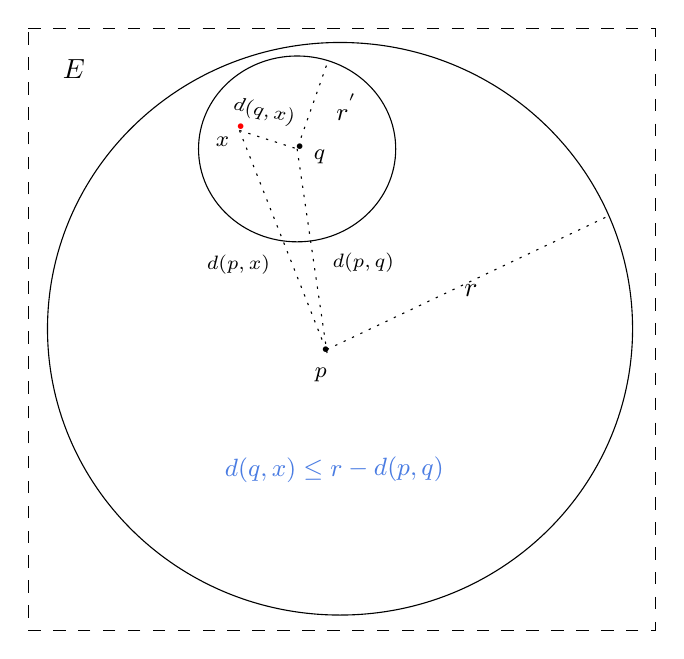
\begin{tikzpicture}[x=0.75pt,y=0.75pt,yscale=-1,xscale=1]
%uncomment if require: \path (0,472); %set diagram left start at 0, and has height of 472

%Shape: Rectangle [id:dp36732556175622055] 
\draw  [dash pattern={on 4.5pt off 4.5pt}] (158.57,81.29) -- (460.57,81.29) -- (460.57,371.29) -- (158.57,371.29) -- cycle ;
%Shape: Ellipse [id:dp4665256155664408] 
\draw   (167.85,226.09) .. controls (167.85,149.91) and (230.95,88.15) .. (308.79,88.15) .. controls (386.63,88.15) and (449.74,149.91) .. (449.74,226.09) .. controls (449.74,302.27) and (386.63,364.02) .. (308.79,364.02) .. controls (230.95,364.02) and (167.85,302.27) .. (167.85,226.09) -- cycle ;
%Straight Lines [id:da9766682347288755] 
\draw  [dash pattern={on 0.84pt off 2.51pt}]  (436.62,172.45) -- (301.2,236.7) ;
%Shape: Ellipse [id:dp01457511604137074] 
\draw   (240.62,139.43) .. controls (240.62,114.7) and (261.89,94.66) .. (288.12,94.66) .. controls (314.35,94.66) and (335.62,114.7) .. (335.62,139.43) .. controls (335.62,164.16) and (314.35,184.2) .. (288.12,184.2) .. controls (261.89,184.2) and (240.62,164.16) .. (240.62,139.43) -- cycle ;
%Straight Lines [id:da776417097753616] 
\draw  [dash pattern={on 0.84pt off 2.51pt}]  (302.22,99.3) -- (288.12,139.43) ;
%Straight Lines [id:da7683663505583478] 
\draw  [dash pattern={on 0.84pt off 2.51pt}]  (260.35,130.54) -- (300.82,233.1) ;
%Straight Lines [id:da24390474713752863] 
\draw  [dash pattern={on 0.84pt off 2.51pt}]  (260.35,130.54) -- (288.12,139.43) ;
%Straight Lines [id:da17965772530026092] 
\draw  [dash pattern={on 0.84pt off 2.51pt}]  (288.12,139.43) -- (302.59,238.19) ;

% Text Node
\draw (367.41,203.72) node [anchor=north west][inner sep=0.75pt]   [align=left] {$\displaystyle r$};
% Text Node
\draw (283.92,135.63) node [anchor=north west][inner sep=0.75pt]  [font=\Huge] [align=left] {.};
% Text Node
\draw (296.76,233.66) node [anchor=north west][inner sep=0.75pt]  [font=\Huge] [align=left] {.};
% Text Node
\draw (305.8,111.43) node [anchor=north west][inner sep=0.75pt]  [font=\small] [align=left] {$\displaystyle r^{'}$};
% Text Node
\draw (255.65,126.25) node [anchor=north west][inner sep=0.75pt]  [color={rgb, 255:red, 255; green, 0; blue, 0 }  ,opacity=1 ] [align=left] {{\Huge .}};
% Text Node
\draw (295.38,243.81) node [anchor=north west][inner sep=0.75pt]  [font=\footnotesize] [align=left] {$\displaystyle p$};
% Text Node
\draw (294.91,138.69) node [anchor=north west][inner sep=0.75pt]  [font=\footnotesize] [align=left] {$\displaystyle q$};
% Text Node
\draw (247.76,132.33) node [anchor=north west][inner sep=0.75pt]  [font=\footnotesize] [align=left] {$\displaystyle x$};
% Text Node
\draw (243.38,189.47) node [anchor=north west][inner sep=0.75pt]  [font=\scriptsize] [align=left] {$\displaystyle d( p,x)$};
% Text Node
\draw (257.67,112.25) node [anchor=north west][inner sep=0.75pt]  [font=\scriptsize,rotate=-12.85] [align=left] {$\displaystyle d( q,x)$};
% Text Node
\draw (304,188.52) node [anchor=north west][inner sep=0.75pt]  [font=\scriptsize] [align=left] {$\displaystyle d( p,q)$};
% Text Node
\draw (252.02,287.1) node [anchor=north west][inner sep=0.75pt]  [font=\small,color={rgb, 255:red, 74; green, 124; blue, 226 }  ,opacity=1 ,rotate=-359.68] [align=left] {$\displaystyle d( q,x) \leq r-d( p,q)$};
% Text Node
\draw (174,95) node [anchor=north west][inner sep=0.75pt]   [align=left] {$\displaystyle E$};


\end{tikzpicture}
        \end{center}
        \begin{proof}
            Sea $x \in B_E(q,r^{\prime})$, entonces;

            \begin{align*}
                d(p,x)&\leq d(p,q)+d(q,x)\\
                &\leq r-d(q,x)+d(q,x)\\
                &\leq r
            \end{align*}

         Luego el punto $x\in B_E(p,r)$ y se tiene la contenencia\\
        \end{proof} 

Note que la prueba no debe depender del dibujo, sin embargo hacer dibujos puede ser de ayuda para tener una idea de la demostración, como ocurrió en este caso

\begin{theorem}[Teorema 9]

Dado $(E,d)$ en espacio métrico, tenemos que:

\begin{itemize}
\item[1)]$E$ es cerrado

\item[2)] $\emptyset$ es cerrado

\item[3)] Unión finita de cerrados es cerrada.

\item[4)]Intersección arbitraria de cerrados es cerrada.

\end{itemize}
\end{theorem}

\begin{proof}
Note que $E^C=$ $\emptyset$ luego el complemento de $E$ es abierto. 
\end{proof}

\begin{proof}
Por definición $E$ es abierto, luego $\emptyset$ es cerrado.
\end{proof}

\begin{proof}
Consideremos $C_i$ una familia de cerrados, luego

$$\left(\bigcup_{i=1}^n C_i\right)^C=\bigcap_{i=1}^n C_i^C$$

Y como intersección finita de abiertos es abierto, entonces acabamos.
\end{proof}

\begin{proof}
Nuevamente consideremos $C_i$ una familia de cerrados, entonces:

$$\left(\bigcap_{i \in I}C_i\right)^C=\bigcup_{i\in I}C_i^C$$

Y como unión arbitraria de abiertos es abierto, entonces acabamos.

\end{proof}

\end{itemize}

\begin{itemize}
\item[✎]Sea $(E,d)$ un espacio métrico $\{p\}=\bigcap_{r>0} B[p, r]$\\

\begin{proof}
Suponga que $\{p\}\neq \bigcap_{r>0} B[p, r]$, luego existe $x\in \bigcap_{r>0} B[p, r]$ tal que $x\neq p$, entonces $x \in B[p,r]$ para todo $r>0$, pero $x\neq p$, por tando $d(x,p)>0$, así existe $0<r<d(x,p)$ tal que $x\not \in B[p,r]$, contradicción.
 \end{proof}
\end{itemize}



\section{Quiz 4:}

\begin{itemize}
\item[✎] \textbf{Falso: }Observamos que vía la definición de abierto $\mathbb{Q}$ no puede ser abierto ya que toda bola con centro en un racional va a tener irracionales dentro que no están en $\mathbb{Q}$ y por tanto la bola no está contenida en $\mathbb{Q}$, luego no es abierto.

De hecho es la forma de argumentar esto, vía la densidad de $\mathbb{Q}$ en $\mathbb{R}$ que ya conocemos de los cursos anteriores.

De manera más formal para todo $r>0$, $B(q,r)=(q-r,q+r) \not \subseteq \mathbb{Q}$, ya que $\mathbb{Q}$ es denso en $\mathbb{R}$.

Esto ocurre ya que estamos tomando bolas en $\mathbb{R}$. (Este argumento es para la métrica usual).

\item[✎] \textbf{Verdadero: } \\
\begin{proof}
    Sea $q \in \mathbb{Q}$, consideremos $B(q,\frac{1}{2})$ entonces como estamos en la métrica discreta $B(q,\frac{1}{2})=\{x\in \mathbb{R}:d_d(q,x)<\frac{1}{2}\}=\{q\}$ por definición de la métrica y como podemos hacer esto para todo $q\in \mathbb{Q}$ y un conjunto es abierto si y solo si es unión de bolas abiertas, razonando inductivamente acabamos.
\end{proof}


\item[✎] \textbf{Verdadero: }$B(0,\frac{1}{2})=\{x\in \mathbb{R} : d_d(0,x)<\frac{1}{2}\}=\{0\}=\{x \in \mathbb{R} : d_d(0,x)\leq \frac{1}{4}\}=B[0,\frac{1}{4}]$

\item[✎]\textbf{Verdadero: }\\
\begin{proof}
    Para ver que los naturales son cerrados con $d_1$, veamos que su complemento es abierto. Observe que:


    $$\displaystyle \mathbb{R}\setminus\mathbb{N}=(-\infty,0)\bigcup_{i \in \mathbb{N}}B\left(i+\frac{1}{2},\frac{1}{2}\right)$$


Note que esas bolas son abiertas y unión arbitraria de abiertos es abierto, efectivamente esas bolas cubren $\mathbb{R}\setminus \mathbb{N}$ entonces acabamos.
    
\end{proof}


\item[✎]\textbf{Verdadero: } \\
\begin{proof}
    Sea $X\subseteq R$ en $(R,d_d)$, $X$ es abierto ya que:

    $$X=\bigcup_{x \in X}B\left(x,\frac{1}{2}\right)$$

    Y $\mathbb{R}\setminus X$ también ya que:

     $$\mathbb{R}\setminus X=\bigcup_{j \in \mathbb{R}\setminus X}B\left(j,\frac{1}{2}\right)$$

     Luego $X$ es cerrado ya que su complemento es abierto, estos conjuntos los llamaremos \textbf{clopen} para simplificar en algunos casos.
\end{proof}

Note que podemos escoger cualquier $r\leq 1$ y la prueba se mantiene.

\item[✎] \textbf{Falso: }Queremos ver que $[0,\frac{1}{4})^C=[\frac{1}{4},\frac{1}{2})$ no es abierto, note que $B(\frac{1}{4},r)=(\frac{1}{4}-r,\frac{1}{4}+r)$ para todo $r>0$ no está contenida en $[\frac{1}{4},\frac{1}{2})$, entonces $[0,\frac{1}{4})$ no es cerrado en $([0,\frac{1}{2}),d|_{[0,\frac{1}{2})\text{x}[0,\frac{1}{2})})$ 

\item[✎] \textbf{Falso: }El conjunto $\left[0, \frac{1}{2}\right)$ es abierto en $\left(\left[0, \frac{1}{2}\right),\left.d_1\right|_{\left[0, \frac{1}{2}\right) \times\left[0, \frac{1}{2}\right)}\right)$, pero no en $(R,d_1)$

\item[✎]\textbf{Verdadero: }\\
\begin{proof}
    Sea $A$ abierto en $(E,d)$, entonces:

    $$A=\bigcup_{a\in A} B(a,r_a)$$

    Luego:

    $$A\cap E_1=\bigcup_{a\in A} B(a,r_a)\cap E_1$$

Y sabemos que $B(a,r_a)\cap E_1$ es abierto en $E_1$ y como unión arbitraria de abiertos es abierto $A\cap E_1$ es abierto, es decir $A$ es abierto en $E_1$.\\
\end{proof}

Y acabamos esta sección.
\end{itemize}

\section{Quiz 5: }

\begin{itemize}
    \item[✎]\textbf{Verdadero: }\\
    \begin{proof}
        Sea $x \in \mathbb{R}$ entonces $(B(x,\frac{1}{3})\setminus \{x\})=\text{\O}$, luego $(B(x,\frac{1}{3})\setminus \{x\})\cap \mathbb{Q}=$\O, por tanto $\mathbb{Q}^{\prime}=$\O.\\ 
    \end{proof}


    \item[✎] \textbf{Falso: }Sabemos que $S$ es cerrado si y solo si $\overline{S}=S$, antes probamos que $\mathbb{N}$ en $(\mathbb{R},d_1)$ es cerrado luego $$\overline{\mathbb{N}}=\mathbb{N}$$


    \item[✎] \textbf{Falso: }Sabemos que $\partial \mathbb{Q}=$$\overline{\mathbb{Q}}\cap$$\overline{\mathbb{R}\setminus\mathbb{Q}}$ y como $\mathbb{Q}$ y $\mathbb{R}\setminus\mathbb{Q}=\mathbb{I}$ son densos en $\mathbb{R}$ entonces $\overline{\mathbb{Q}}=\mathbb{R}$ y $\overline{\mathbb{I}}=\mathbb{R}$, así $\partial \mathbb{Q}=\mathbb{R}$


    \item[✎] \textbf{Verdadero: }\\
    \begin{proof}
        Tenemos que $x \in [0,1)^{\prime}$ si y solo si $x \in \overline{[0,1)-\{x\}}$, observe que:
        
        \begin{align*}
            \overline{[0,1)-\{x\}}&=[0,1)\setminus int([0,1]\setminus ([0,1)\setminus \{x\}))\\
            &=[0,1)\setminus int(\{x\})\\
            &=[0,1)\setminus \text{\O}
        \end{align*}
        
        En efecto si $x\in [0,1)$, $x \in [0,1)^{\prime}$ 
    \end{proof}

    \item[✎]\textbf{Verdadero: }$\partial \mathbb{R}=$$\overline{\mathbb{R}}\cap$$\overline{\text{\O}}=\mathbb{R}\cap$\O$=$\O


    \item[✎]\textbf{Verdadero: } \\
    \begin{proof}
        Como en las pruebas anteriores note que si $r\leq1$ entonces para todo $x\in \mathbb{R}$, $B(x,r)\setminus\{x\}=$$\emptyset$ y por tanto $B(x,r)\setminus\{x\}\cap \mathbb{R}=$\O, luego $\mathbb{R}^{\prime}=$\O
    \end{proof}


    \item[✎] \textbf{Falso: }Sea $(\mathbb{R},d_d)$ los reales con la métrica discreta, luego:

    $$\overline{B(0,1)}=\overline{\{0\}}=\{0\}$$

Mientras que:

$$B[0,1]=\mathbb{R}$$

    \item[✎]\textbf{Verdadero: }\\
    \begin{proof}
        Tenemos que: 

    $$
d_1(p, q)=\sum_{k=1}^n\left|p_k-q_k\right|
$$
$y$
$$
d_{\infty}(p, q)=\operatorname{máx}_{1 \leq k \leq n}\left|p_k-q_k\right| .
$$

Pero como en este caso estamos en $\mathbb{R}$, entonces 

$$
d_1(p, q)=|p-q|=d_{\infty}(p,q)
$$

Entonces como $\mathbb{N}$ es cerrado en $(\mathbb{R},d_1)$, tambien es cerrado en $(\mathbb{R},d_{\infty})$

    \end{proof}

    \item[✎]\textbf{Verdadero: }\\
    
   \begin{proof}
         Tenemos que $A$ es cerrado en $(\mathbb{R}^n,d_{\infty})$, luego $A^C$ es abierto en $(\mathbb{R}^n,d_{\infty})$, así para todo $x\in A^C$ existe un $r_x$ tal que:

         $$B_{\infty}(x,r_x)=\{y\in \mathbb{R}^n: d_{\infty}(x,y)<r_x\}\subseteq A^C$$

         Ahora supongamos que $A$ no es cerrado en $(\mathbb{R}^n,d_1)$, luego $A^C$ no es abierto en $(\mathbb{R}^n,d_1)$, es decir, existe $a \in A^C$ tal que para todo $r>0$:

         $$B_2(a,r)\not \subseteq A^C$$

         En particular $B_2(a,r_a)\not \subseteq A^C$, pero como $d_{\infty}(x,y)\leq d_2(x,y)<r_a$, entonces $B_2(a,r_a)\subseteq B_{\infty}(a,r_a)\subseteq A^C$, contradicción.
         
    \end{proof}
    
   

    
\end{itemize}
\vspace{0.3cm}
 \section{Ejercicios adicionales.}
    
\begin{note}
 los siguientes ejercicios fueron propuestos en 2022-2 en un parcial de Análisis, el propósito de esta sección es que sirva para que el estudiante pueda hacerse una idea del modelo de preguntas que se suelen hacer y esté preparado
\end{note}


\begin{itemize}

\item[]\textbf{En cada caso determine si el enunciado es verdadero o falso. Si es verdadero demuéstrelo de lo contrario dé un contra ejemplo.}

    \item[☠]Si $A \neq \varnothing$ es un subconjunto cerrado y acotado inferiormente en $\mathbb{R}$ con la métrica usual $|x-y|$ entonces $A$ tiene elemento mínimo.\\
    
    \textbf{Verdadero:}\\
    
    \begin{proof}
        Supongamos que $A$ es acortado inferiormente en $\mathbb{R}$, entonces exite $i=\inf(A)$, veamos que $i\in A$. Supongamos que $i \not \in A$, entonces $i \in \mathbb{R}\setminus A$, $\mathbb{R}\setminus A$ es abierto porque $A$ es cerrado, entonces exite $\epsilon>0$ tal que $B(i,\epsilon)=(i-\epsilon,i+\epsilon)\subseteq \mathbb{R}\setminus A$, por otro lado como $i=\inf(A)$ existe $b\in A$ tal que $i\leq b< i+\epsilon$, luego $b\in (i-\epsilon,i+\epsilon)\subseteq \mathbb{R}\setminus A$. Contradicción, luego $i \in A$, es decir $i=\min(A)$.
        
    \end{proof}
    
    \item[☠]Sean $(X, d)$ un espacio métrico y $A, B$ subconjuntos de $X$ tales que $int($$A) \subseteq B \subseteq \bar{A}$ entonces $\bar{B}=\bar{A}$.\\
    
    \textbf{Falso: }Contraejemplo: Sean $(\mathbb{R},d_1)$, $\mathbb{N}=A$ y $\{0\}=B$, entonces como $int(\mathbb{N})=$\O, es claro que $int(\mathbb{N})\subseteq\{0\}$, por otro lado $\overline{\mathbb{N}}=\mathbb{N}$ ya que $\mathbb{N}$ es cerrado, y $\overline{\{0\}}=\{0\}$, en efecto $\{0\}\neq \mathbb{N}$.
    
    \item[☠]Si $(X, d)$ es un espacio métrico entonces $d^{\prime}(x, y)=d^2(x, y)$ también define una métrica en $X^2$.
    
    \textbf{Falso: }Contraejemplo: Tome $(\mathbb{R},d_1)$, veamos que $(\mathbb{R},d_1^2)$ no es un espacio métrico. Note que $d_1^2(3,1)>d_1^2(3,2)+d_1^2(2,1)$ $(4>1+1)$, lo que contradice la desigualdad triangular
    
    \item[☠]$(X, d)$ un espacio métrico y $\left(A_j\right)_{j \in J}$ una familia de subconjuntos de $X$. Si $a \in \overline{A_j}$ para todo $j \in J$ entonces $a \in \overline{\bigcap_{j \in J} A_j}$.\\
    
    \textbf{Falso: }Contrajemplo: Sean $\mathbb{Q}, \mathbb{I}$, en $(\mathbb{R},d_1)$, y sea $x=\sqrt{2}$, como $\overline{\mathbb{Q}}=\overline{\mathbb{I}}=\mathbb{R}$, $x \in \overline{\mathbb{Q}}$ y $x\in \overline{\mathbb{I}}$, sin embargo $x\not \in \overline{\mathbb{Q}\cap \mathbb{I}}=\overline{\text{\O}}=$\O

    
    \item[☠☠] Sean:
    \begin{itemize}
        
\item $X$ el espacio de las funciones acotadas $f: I \rightarrow \mathbb{R}$ definidas en el intervalo real $I=[0,1]$,

\item $d$ la métrica definida en $X^2$ por $d(f, g)=\sup _{x \in I}|f(x)-g(x)|$,

\item $f_0(x)=x^2, f_n(x)=\dfrac{x^2 \operatorname{sen}(2 \pi n x)}{2 \pi n}                       
    \operatorname{con} n \in \mathbb{Z}^{+}, x \in I$ y

\item $B\left(f_0, \frac{3}{2}\right)=\left\{f \in X: d\left(f, f_0\right)<\frac{3}{2}\right\}$
entonces $f_n \in B\left(f_0, \frac{3}{2}\right)$ para todo $n \in \mathbb{Z}^{+}$.\\

    \end{itemize}
   
 \begin{proof}
    Queremos ver que $f_n\in B(f_0,\frac{3}{2})$ para todo $n \in \bb{Z}^+$, es decir que $d(f_n,f_0)<\frac{3}{2}$ para todo $n \in \bb{Z}^+$, luego por la definición de la métrica:
    
    \begin{align*}
        d(f_n,f_0)&=\sup_{x \in I}\left|x^2-\dfrac{x^2sen(2\pi nx)}{2\pi n}\right|\\
        &=\sup_{x \in I}\left|x^2\left(1-\dfrac{sen(2\pi nx)}{2\pi n}\right)\right|\\
        &\leq\sup_{x \in I}\left|1-\dfrac{sen(2\pi nx)}{2\pi n}\right| && (x^2\leq 1)\\
        &\leq\left|1-\dfrac{1}{2\pi n}\right|&&(-1\leq sin(\theta)\leq 1)\\
        &\leq \dfrac{3}{2}\\
        &=1.5
     \end{align*}

Ya que $0<\frac{1}{2\pi n}< 1$ para todo $n \in \Z^+$

    
\end{proof}  
   
   \begin{note}
   cuando decimos métrica sobre $X^2$ queremos decir que la métrica va del producto cartesiano $X \text{ x } X$ en $\bb{R}$, no confundir con $X^2 \text{ x } X^2$ 
   \end{note}
   


\begin{note}
Los siguientes ejercicios fueron propuestos en 2023-1 en el primer parcial de análisis:
\end{note}

\end{itemize}


Sean $(X, d)$ es un espacio métrico y $A$ es un subconjunto de $X$. En cada caso determine si la proposición es verdadera o falsa y demuéstrela o dé un contra-ejemplo según sea el caso.

\begin{itemize}[label={☠}]
\item $X=\overline{A}\cup A^{C}$\\

\begin{proof}
Sabemos que $\overline{A}=X\setminus int(A^C)$. En efecto $X\setminus int(A^C)\cup A^C=X$ ya que $int(A^C)\subseteq A^C$
\end{proof}
 
\item $\partial(\partial A)=\partial A$\\

\textbf{Falso:} Contraejemplo: Considere $(\R,d_1)$, sabemos que $\partial \Q=\R$ y que $\partial \R= $\O, luego $\partial \Q=\R\neq\partial(\partial \Q)=\partial \R=$\O

\item $X=int(A)\cup \partial(A) \cup A^C$\\

\begin{proof}
Tenemos que $\partial A=\bar{A} \cap \overline{A^C}$, luego

\begin{align*}
int(A)\cup (\overline{A}\cap \overline{A^C}) \cup A^C&=int(A)\cup (\overline{A}\cup A^C\cap \overline{A^C}\cup A^C)\\
&=int(A)\cup (X\cap (X\setminus int(A)\cup A^C))\\
&=int(A)\cup (X\setminus int(A))\\
&=X
\end{align*}
\end{proof}

\begin{note}
Aquí usamos varias de las propiedades de las notas en el capítulo del concepto de clausura, derivado y frontera, note que además usamos la propiedad anterior en la prueba cuando afirmamos que $\overline{A}\cup A^C=X$, note también que usamos que $(A^C)^C=A$ pero pues ustedes ya vieron conjuntos allí.
\end{note}

\item $int(int(A))=int(A)$\\

\begin{proof}
 Tenemos que $int(A)$ es abierto, luego como un conjunto es abierto si y solo si es igual a su interior entonces $int(int(A))=int(A)$
\end{proof}


\item Si $\partial A$ es abierto entonces $A=$\O\\

\textbf{Falso:} Contraejemplo: Considere $(R,d_1)$, luego $\partial \Q=\R$ y $\R$ es abierto pero $\Q\neq$\O.



\item Si $X=\mathbb{R}^n$ y $A$ es $d_1$-abierto entonces $A$ es $d_2$-abierto.\\

\begin{proof}
Suponga que $A$ es $d_1$-abierto, entonces para todo $x\in A$, existe $r$ tal que:

$$B_1(x,r)=\{y\in \R^{n} : d_1(x,y)<r\}\subseteq A$$

Y como $d_2(x,y)\leq d_1(x,y)$, entonces existe $r^{\prime}$ $B_2(x,r^{\prime})\subseteq B_1(x,r)\subseteq A$, luego $A$ es $d_2-$abierto

\end{proof}

\begin{note}
Para este caso estamos usando la definición de métrica equivalente, note que si $d_2(x,y)\leq d_1(x,y)$ entonces exiete $C\in \R$ tal que $d_1(x,y)\leq C d_2(x,y)$, luego eso es lo que nos garantiza la exitencia de ese radio $r^{\prime}$ de tal manera que $B_2(x,r^{\prime})\subseteq B_1(x,r)$. 
\end{note}

\begin{note}
Note que en las notas hace falta hacer énfasis en esta definición, sin embargo este tipo de detalles se suelen cubrir en clase, en cualquier caso el lector puede buscar en algún medio externo la definición de métrica equivalente y notar este detalle sutil.
\end{note}



\item Si $A \subseteq Y \subseteq X$ y $A$ es $Y$-abierto entonces $A$ es $X$-abierto.\\

\textbf{Falso: } Contraejemplo: Si $E=\mathbb{R}$ con $d(x, y)=|x-y|$ el conjunto $\left[0, \frac{1}{3}\right)$ no es abierto en $\mathbb{R}$ pero es abierto en $\left(E_1,\left.d\right|_{E_1 \times E_1}\right)$ con $E_1=\left[0, \frac{1}{2}\right)$. Simplemente observe que $B_{E_1}\left(0, \frac{1}{3}\right)=\left[0, \frac{1}{3}\right)$.

\item Si $x \in X$ entonces para todo $r>0$ se tiene que $\overline{B(x, r)}=B[x, r]$.\\

\textbf{Falso:} Contraejemplo: Sea $(\R,d_d)$, entonces $\overline{B(0,1)}=\overline{\{0\}}=0$ ya que $\{0\}$ es cerrado con la métrica discreta, pero $B[0,1]=\R$, luego no son iguales.

\end{itemize}

\begin{note}
Sobre este parcial como se puede notar los ejercicios no son tan complejos si se nos permite usar las propiedades de las notas (que se ven también en clase), pero es probable que para ser usadas en el parcial el estudiante deba demostrarlas, en cuyo caso recomendamos entender muy bien las ideas de cada una de las pruebas, la idea nunca es memorizar las pruebas o las propiedades sino entender un poco la geometría del asunto y las ideas principales de cada prueba.
\end{note}

\section{El conjunto de Cantor ☠☠☠☠☠ }